% http://theoval.cmp.uea.ac.uk/~nlct/latex/pdfdoc/pdfdoc/pdfdoc.html
% http://vavricek.cs.vsb.cz/index.php/LaTeX/Vychyt%C3%A1vky
% http://vavricek.cs.vsb.cz/index.php/LaTeX
% http://phoenix.inf.upol.cz/propedeutika/2/practice1.html

% http://www.tex.ac.uk/cgi-bin/texfaq2html?label=newlang nějaká hláška z babelu, jak se zbavit warningu -nefunguje mi :(

\documentclass[
	12pt, 												% velikost písma
	%fleqn, 											% zarovnání rovnic do leva
	leqno, 												% číslování rovnic vlevo
	oneside, 											% jednostranný tisk
	%twoside,											% oboustranný tisk
]{article}											% articke neumí kapitoly, pokud budou potřeba, použít: report / article
%Options -- Point size:  10pt (default), 11pt, 12pt
%        -- Paper size:  letterpaper (default), a4paper, a5paper, b5paper
%                        legalpaper, executivepaper
%        -- Orientation  (portrait is the default)
%                        landscape
%        -- Print size:  oneside (default), twoside
%        -- Quality      final(default), draft
%        -- Title page   notitlepage, titlepage(default)
%        -- Columns      onecolumn(default), twocolumn
%        -- Equation numbering (equation numbers on the right is the default)
%                        leqno
%        -- Displayed equations (centered is the default)
%                        fleqn (equations start at the same distance from the right side)
%        -- Open bibliography style (closed is the default)
%                        openbib
% For instance the command
%           \documentclass[a4paper,12pt,leqno]{article}
% ensures that the paper size is a4, the fonts are typeset at the size 12p
% and the equation numbers are on the left side
%

\usepackage[a4paper,inner=4cm,outer=2.5cm]{geometry} % velikost vnějšího okraje stránek
\usepackage[a4paper]{geometry}  % velikost vnějšího okraje stránek
%\usepackage{a4wide} 						% nastaví velikost A4 dle evropských (tedy i našich) rozměrů - nefunguje mi :/

%\usepackage[cp1250]{inputenc} 	% jak kódovat české znaky
\usepackage[utf8]{inputenc}

\usepackage[czech]{babel} 			% nastavuje zásady typografie pro českou sazbu pomocí BABELu
\languageattribute{czech}{split}% české dělení textu, http://home.ef.jcu.cz/~houda/miktex/install/babel-cslatex.html

%\ifpdf % Pokud se překládá do PDF... vlastně vždy tisknu do pdf...
\usepackage{cmap}								% % Zajistí správné zakódování národních znaků při výstupu do PDF. Make PDF files search­able and copy­able
%\usepackage{mmap}							% ex­ten­sion of cmap with im­proved flex­i­bil­ity and cov­er­age, in­clud­ing the abil­ity to re-en­code Knuth’s ba­sic math­e­mat­ics fonts.
%\fi % Konec výhradní sekce pro překlad do PDF.

% Pro nastavení písma se musí nastavit fontenc na uvedený u písma a následně písmo, nejlépe písma začínající il2xxxx.fd
%\usepackage[IL2]{fontenc} 			% fonty vyladěné pro češtinu (obávám se, že je to nepoužívá :()
\usepackage{lmodern}						% nejlepší fonty pro čsštinu pro PDF i PS http://home.ef.jcu.cz/~houda/miktex/install/babel-cslatex.html
%\usepackage[T1]{fontenc} 			% rozšíření originálních Knuthových Computer Modern (CM) fontů pro potřeby evropských jazyků psaných latinkou. pro české texty není doporučeno

%\renewcommand{\familydefault}{pbk} % serifové zakulacené
%\renewcommand{\familydefault}{pcr} % používá T1
%\renewcommand{\familydefault}{phv} % bezserifové
%\renewcommand{\familydefault}{ppl} % serifové, hranatější serify

\usepackage[nottoc,notindex,notlof]{tocbibind}					% přidá do obsahu Bibliografii a další http://www.ctan.org/tex-archive/macros/latex/contrib/tocbibind
\usepackage[pdftex,colorlinks=true, unicode=true,breaklinks]{hyperref} % obarvování a aktivování odkazů, pro tisk vypnout
\usepackage{datetime}           % umožní vložení času do hlavičky: http://theoval.cmp.uea.ac.uk/~nlct/latex/packages/datetime/datetime-manual.html
\usepackage{dcolumn}						% zarovnanie cisiel v tabulke podla des. ciarky
\usepackage{enumerate}          % možnost použít \begin{enumerate}[a)] pro písmenný seznam a další (http://www.ctan.org/tex-archive/macros/latex/required/tools/enumerate.pdf)
\usepackage{graphicx} 					% pro vkládání obrázků (optional arguments to the \in­clude­graph­ics command http://www.ctan.org/pkg/graphicx)
\usepackage{listings}						% zobrazení zdrojových kódů pomocí lstlisting (verbatim asi ne)
\usepackage{url} 								% tends to give much more nicely formatted web addresses
\usepackage{verbatim} 					% pro použití víceřádkových komentářů
\usepackage{nomencl}						% [intoc] použiváno pro generování zkratek použitých v dokumentu http://www.ctan.org/pkg/nomencl ("%tm".nlo -s nomencl.ist -o "%tm".nls stáhnout makeindex/nomencl/nomencl.ist)
%\makeglossary									% vygeneruje cosi se zkratkama
\makenomenclature								% vygeneruje soubor se zkratkama
\makeindex											% vygeneruje seznam zkratek

%\usepackage{ae}								% balik pro konverzi sedmibitovych fontu na osmibitove
																% (aby slo pouzit deleni slov http://www.abclinuxu.cz/poradna/linux/show/103978
																% http://www.root.cz/clanky/jak-na-latex-literatura/nazory/
%\usepackage{indentfirst} 			% odsadi i prvni odstavec v textu
%\usepackage{xfrac}             % pro sazbu matematických zlomků pomocí \sfrac{}{}
%\usepackage{natbib}            % sazba pouzite literatury
%\usepackage{amsmath}						% Matematický doplněk http://www.ctan.org/pkg/amsmath
%\usepackage{amsfonts}					% fonts for use in math­e­mat­ics http://www.ctan.org/pkg/amsfonts
%\usepackage{amssymb}						%

\frenchspacing 									% aktivuje použití některých českých typografických pravidel
\pagenumbering{arabic} 					% arabské čísla stránek

% Zobrazení PDF jako single page
\pdfcatalog{/PageLayout /SinglePage}
%\pdfcatalog{/PageLayout /TwoPageRight}

\hypersetup{										% obsah popisu PDF souboru
	baseurl={http://mtrakal.cz},
	pdfkeywords={diplomová práce, mtrakal, Matěj Trakal, cloud},
	pdftitle={Analýza možností nasazení Cloud computing},
	pdfauthor={Matěj Trakal},
	pdfsubject={Diplomová práce}
}

\title{Analýza možností nasazení Cloud computing}
\author{Matěj Trakal}
\date{Poslední úprava: \today}

%\usepackage{fancyhdr} 					% hlavičky dokumentů - http://andy-roberts.net/misc/latex/latextutorial8.html
%%%%%%%%%%%%%%%%%% Změna stylu hlavičky %%%%%%%%%%%%%%%%%%
\begin{comment}
	\lhead{\fancyplain{}INEPD 2010 (Hudec)}
	\lfoot{\fancyplain{}{Matěj Trakal -- \href{http://fei.trtkal.net}{fei.trtkal.net}}}
	\cfoot{\fancyplain{}}
	\rfoot{\fancyplain{}{\thepage}}
	\renewcommand{\footrulewidth}{0.5pt}
\end{comment}
%%%%%%%%%%%%%%%%%% Změna stylu hlavičky %%%%%%%%%%%%%%%%%%

%-------------------------------------------

\begin{document}
\renewcommand{\baselinestretch}{1.1} 			% velikost řádkování

\lstset{language=PHP,basicstyle=\footnotesize,frame=leftline,showspaces=false,showstringspaces=false,showtabs=false}	% nastavení defaultního jazyka a velikosti písma ve zdrojácích

\pagestyle{empty} 												% změní styl od nynější stránky dál do konce dokumentu
	\begin{comment}
		plain - bez číslování stránek 
		empty - potlačí sazbu hlavičky i patičky stránky 
		headings - umístí proměnnou hlavičku na každou stránku. Obsah hlavičky je udán v~dokument style. 
		myheadings - můžete si nadefinovat vlastní hlavičku, a to za pomocí příkazů \markboth nebo \markright
	\end{comment}

% Desky pro tištěnou verzi
\begin{titlepage}
\renewcommand{\baselinestretch}{1} % velikost ��dkov�n�
\begin{center}

\Large\sc
Univerzita Pardubice\\
Fakulta elektrotechniky a informatiky\\[90mm]

{\Huge{\sc{Diplomov� pr�ce}}}\\[90mm]

2013 \hfill Mat�j Trakal

\begin{comment}
	%\flushleft\huge2010\flushright\huge Mat�j Trakal\\
	\begin{tabular}{lp{7cm}r}
	2013 && Mat�j Trakal
	\end{tabular}
\end{comment}


\end{center}
\end{titlepage} % zde kon�� �vodn� strana
\normalsize % nastaven� norm�ln� velikosti fontu






\begin{comment}
	\newpage
	\begin{titlepage} % zde kon�� �vodn� strana
	{\Large\bf Anal�za mo�nost� nasazen� Cloud computing}\\ % dopl�te n�zev pr�ce
	\vspace{5mm}
	???Katedra informa�n�ch technologi�\\ % dopl�te n�zev katedry �i �stavu
	\end{center}
	\vspace{15mm}
	
	\large
	\noindent Vedouc� bakal��sk� pr�ce: ??? Josef Hor�lek % dopl�te odpov�daj�c� �daje
	%%% dal�� ��dek m��ete ve v�t�in� p��pad� (tj. pokud �daje uveden� v��e nejsou p��li� dlouh�) zru�it
	
	???Katedra softwarov�ch technologi�
	\vspace{1mm} 
	
	\noindent Studijn� program: Informa�n� technologie % dopl�te odpov�daj�c� �daje
	%%% dal�� ��dek m��ete ve v�t�in� p��pad� (tj. pokud �daje uveden� v��e nejsou p��li� dlouh�) zru�it
	% \hskip20mm oboru (sm�ru),  p��p. n�zev studijn�ho pl�nu
	
	\vspace{20mm}
	
	\begin{center}
	2010 % dopl�te rok vzniku va�� bakal��sk� pr�ce
	\end{center}
	
	\end{titlepage} % zde kon�� �vodn� strana
	\normalsize % nastaven� norm�ln� velikosti fontu
\end{comment}

% Úvodní strana
\setcounter{page}{1} 											% nastaví číslování od této pozice na číslo
%\begin{titlepage}
%\thispagestyle{empty} % tato stránka nebude mít v zápatí číslo

\renewcommand{\baselinestretch}{1} % velikost řádkování
\begin{center}

\Large\sc
Univerzita Pardubice\\
Fakulta elektrotechniky a informatiky\\[70mm]


\Huge\sc
Analýza možností nasazení Cloud computing\\[20mm]

Matěj Trakal\\[55mm]


\Large\sc
Diplomová práce\\
2014\\
\end{center}
%\end{titlepage} % zde končí úvodní strana
\normalsize % nastavení normální velikosti fontu
\newpage

% Zadání Bc. práce (oskenované)
%\begin{titlepage}
%\thispagestyle{empty} % tato str�nka nebude m�t v z�pat� ��slo

% Zad�n� Bc. pr�ce (oskenovan�)
%\includegraphics[scale=0.3]{logo.eps}

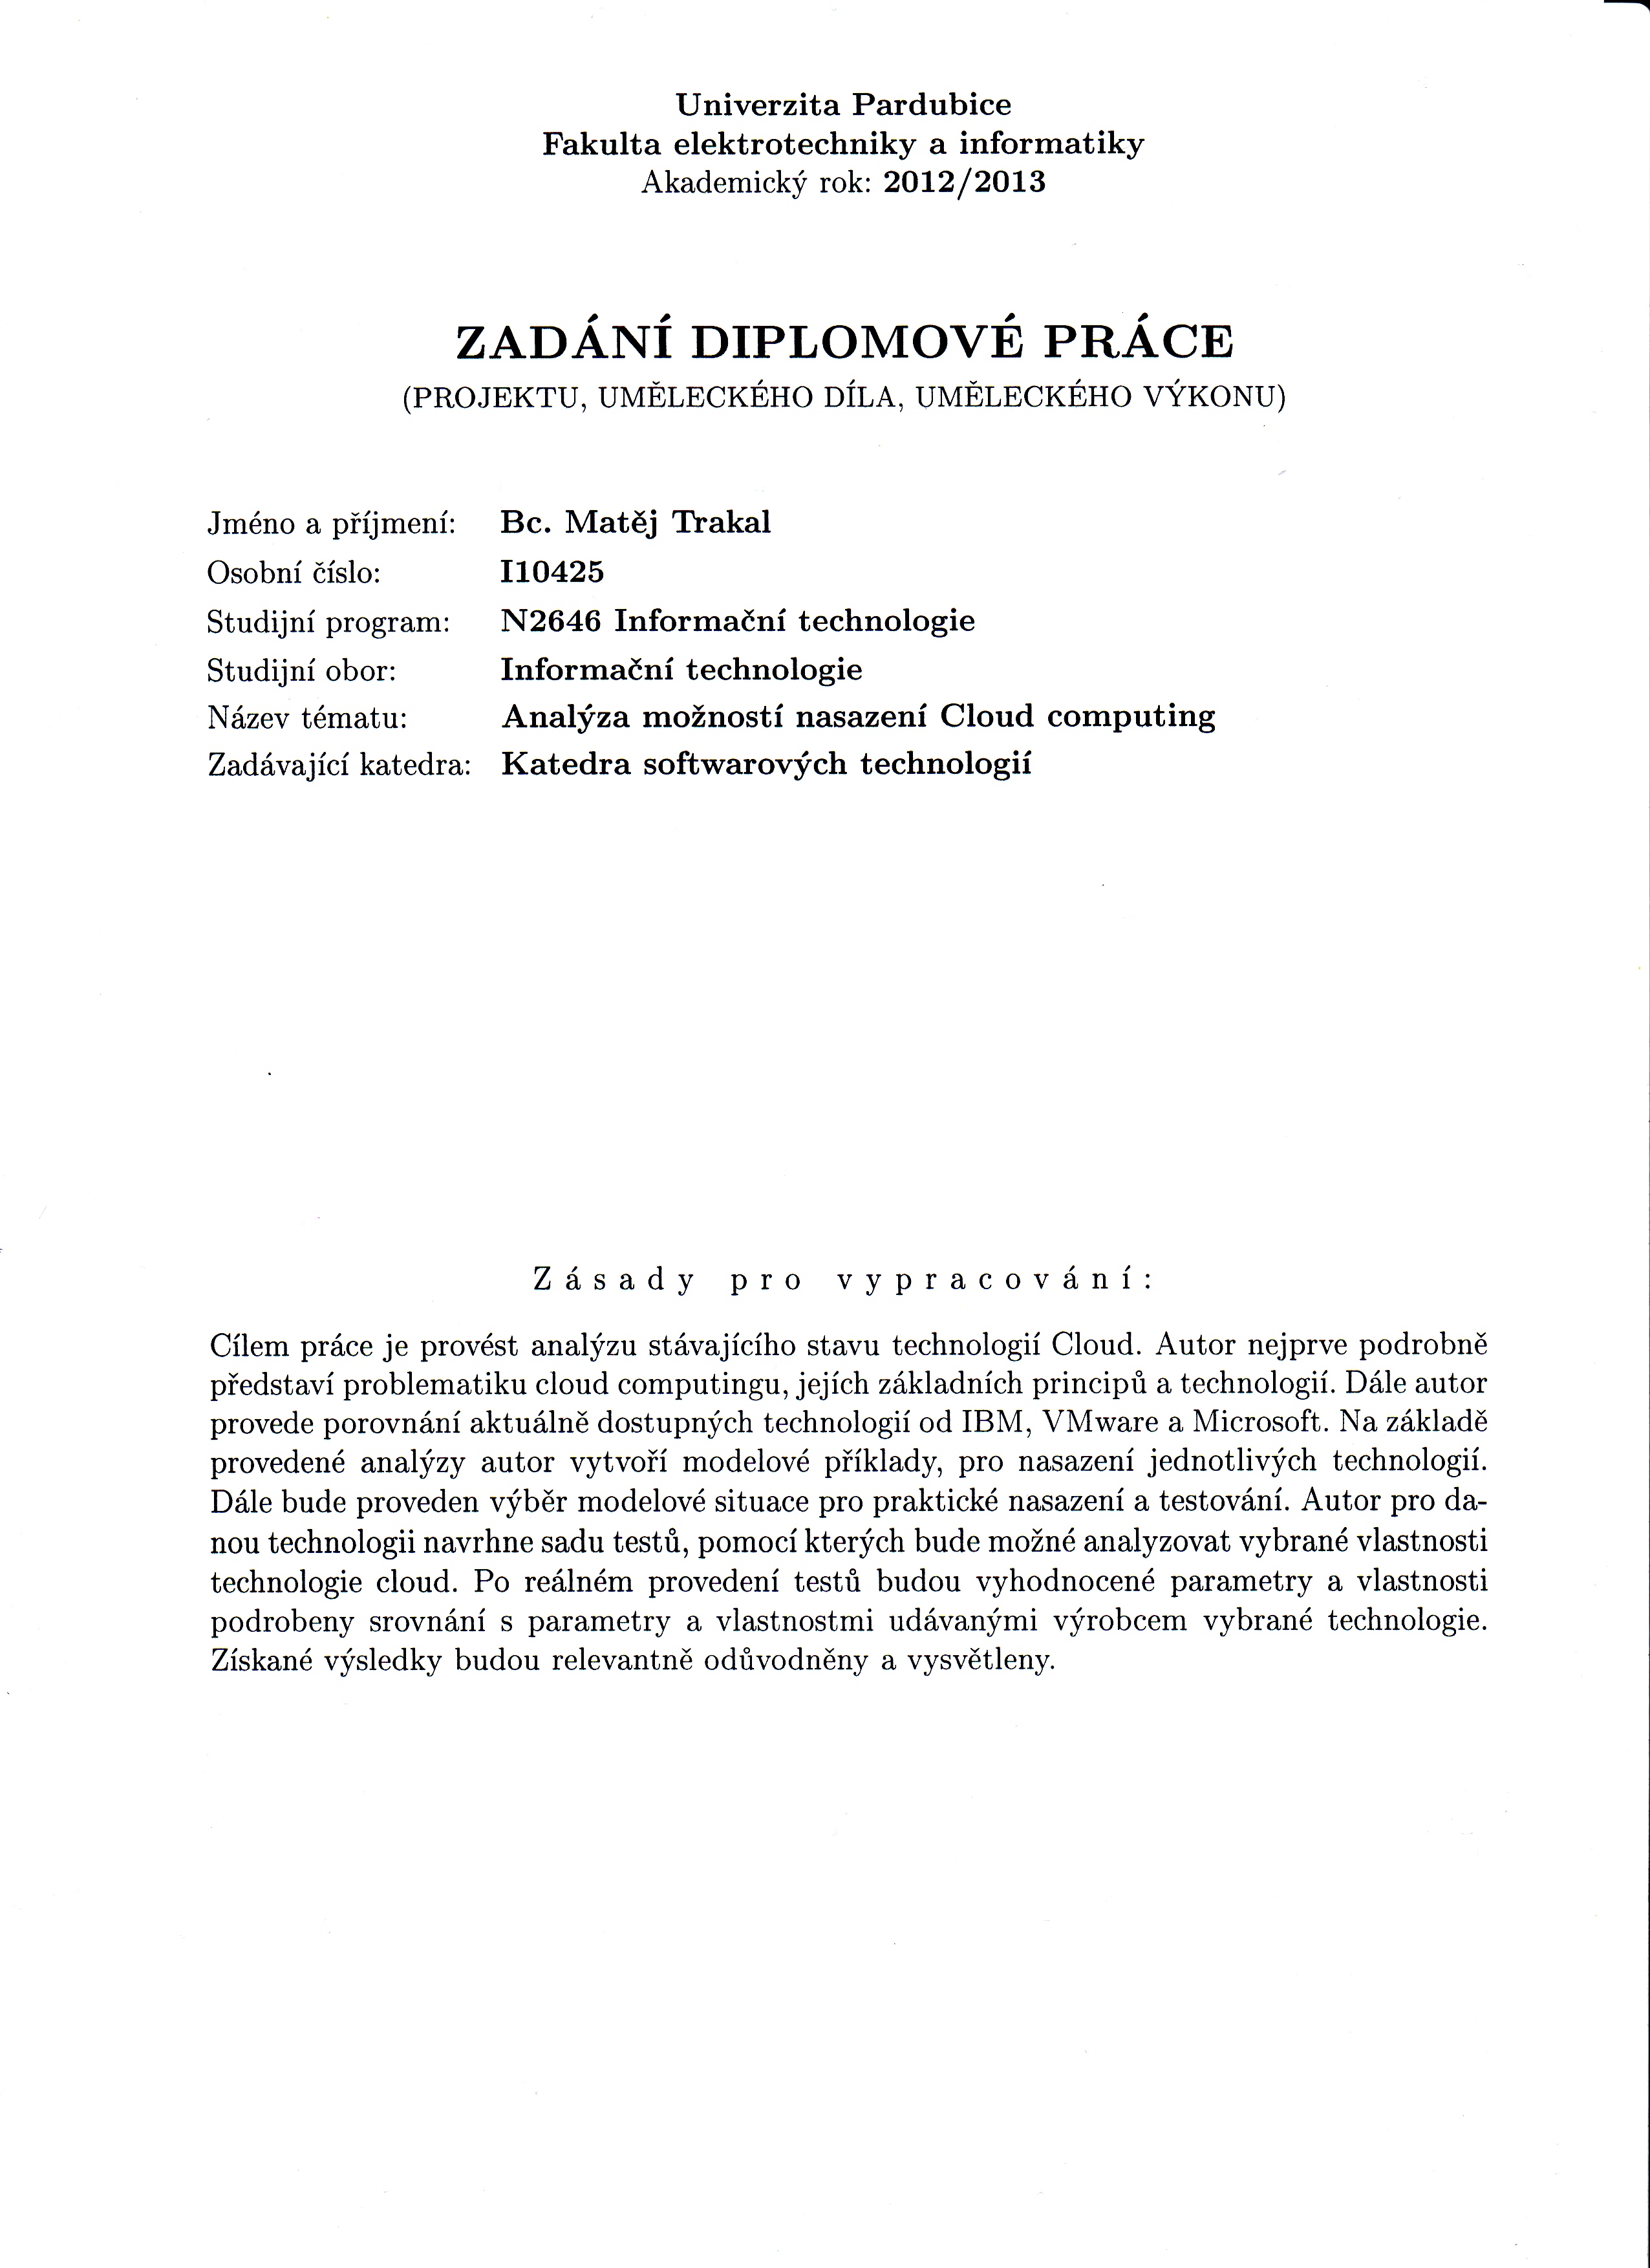
\includegraphics[width=0.95\textwidth]{ext/dp_zad01.png}
% width=1.0\textwidth
\newpage

%\end{titlepage}
%\begin{titlepage}
\thispagestyle{empty} % tato str�nka nebude m�t v z�pat� ��slo
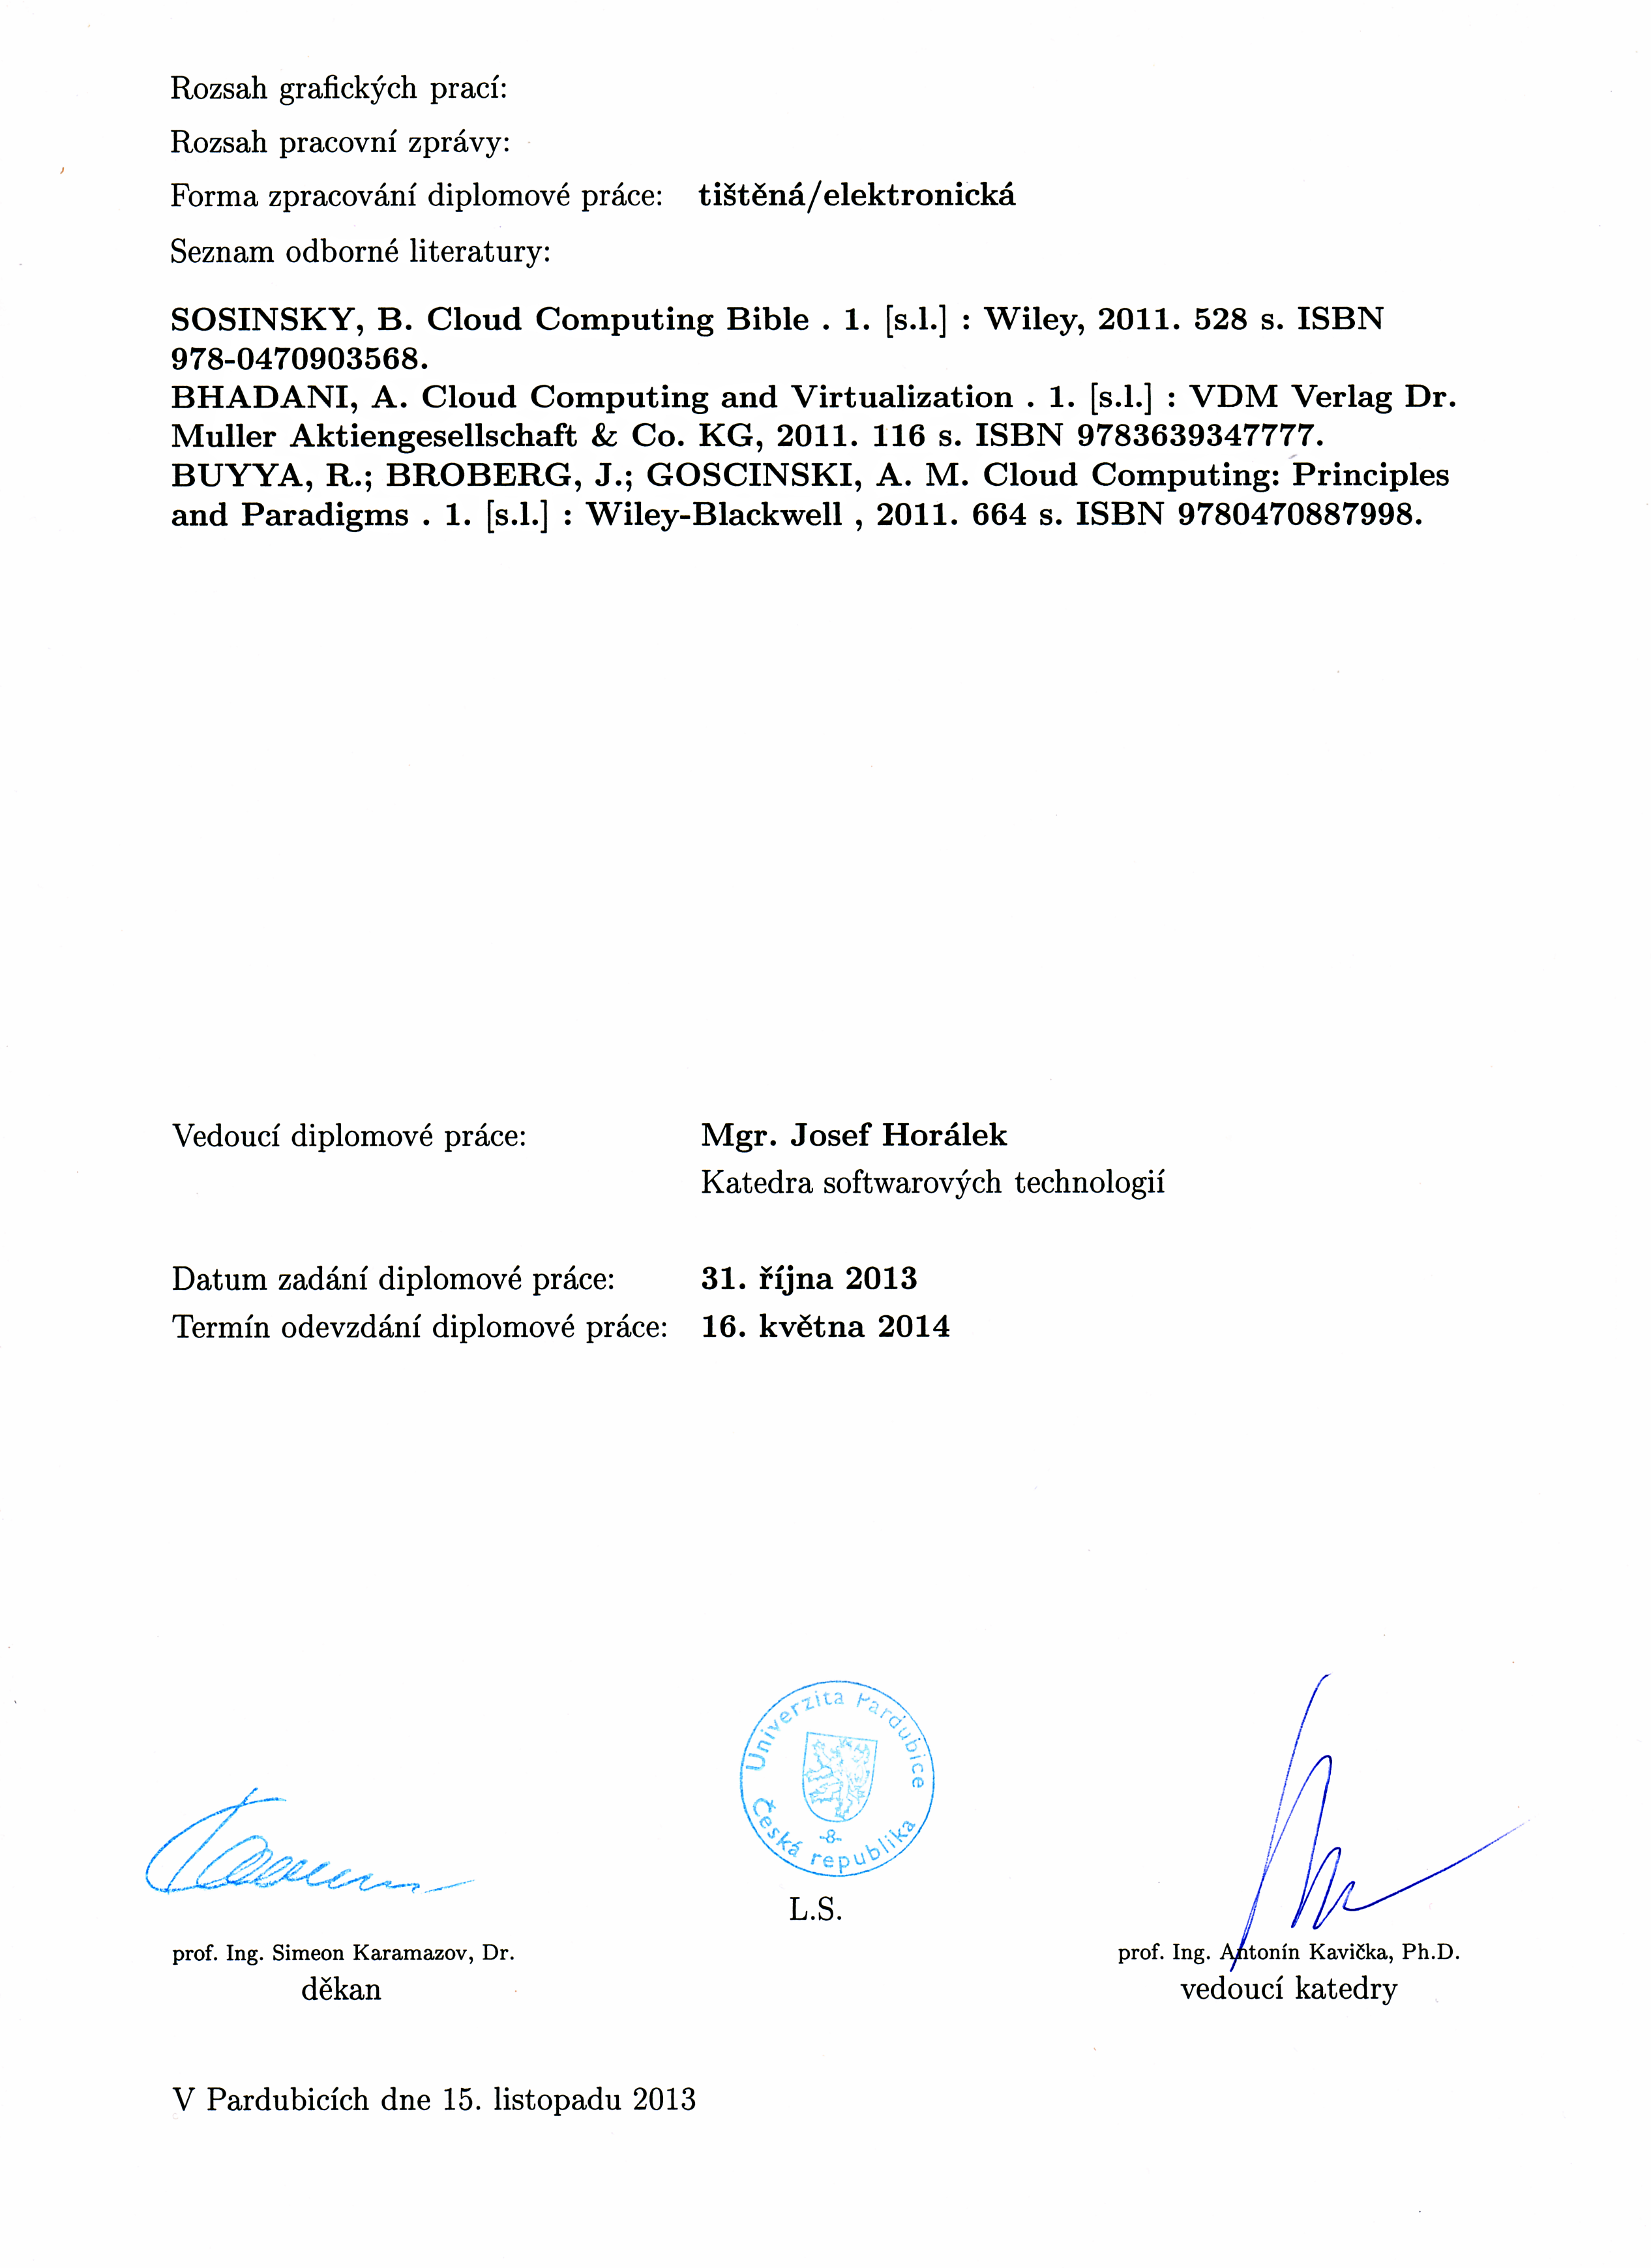
\includegraphics[width=0.95\textwidth]{ext/dp_zad02.png}

%\end{titlepage}
\newpage

\renewcommand{\baselinestretch}{1.1} 			% velikost řádkování
% Prohlášení autora
%\begin{titlepage}
%\thispagestyle{empty} % tato str�nka nebude m�t v z�pat� ��slo

\noindent Prohla�uji:
\vspace{12pt}

Tuto pr�ci jsem vypracoval samostatn�. Ve�ker� liter�rn� prameny a informace, kter� jsem v~pr�ci vyu�il, jsou uvedeny v~seznamu pou�it� literatury.
\vspace{12pt}

Byl jsem sezn�men s~t�m, �e se na moji pr�ci vztahuj� pr�va a povinnosti vypl�vaj�c� ze z�kona �. 121/2000 Sb., autorsk� z�kon, zejm�na se skute�nost�, �e Univerzita Pardubice m� pr�vo na uzav�en� licen�n� smlouvy o~u�it� t�to pr�ce jako �koln�ho d�la podle � 60 odst. 1 autorsk�ho z�kona, a s~t�m, �e pokud dojde k~u�it� t�to pr�ce mnou nebo bude poskytnuta licence o~u�it� jin�mu subjektu, je Univerzita Pardubice opr�vn�na ode mne po�adovat p�im��en� p��sp�vek na �hradu n�klad�, kter� na vytvo�en� d�la vynalo�ila, a to podle okolnost� a� do jejich skute�n� v��e.
\vspace{12pt}

Souhlas�m s~prezen�n�m zp��stupn�n�m sv� pr�ce v~Univerzitn� knihovn�.
\vspace{12pt}

V~Pardubic�ch dne \today

\vspace{24pt}
\begin{flushright}
Mat�j Trakal
\end{flushright}

%\end{titlepage}
\normalsize
\newpage

% Poděkování
%\begin{titlepage}
%\thispagestyle{empty} % tato stránka nebude mít v zápatí číslo
%\noindent{\Large Poděkování}

% !!!
% pokud najdu jak, tak \vspace{180mm}
% !!!

\section*{Poděkování}
Tímto bych chtěl poděkovat Ing.\,Josefu Horálkovi, vedoucímu mé diplomové práce, za jeho velmi cenné rady, pomoc při tvorbě tohoto textu a čas, po který se mi věnoval.

%\end{titlepage}
\newpage

% Abstrakt / Souhrn
%\thispagestyle{empty}

\section*{Souhrn}
Tato pr�ce je zam��ena na ot�zku nasazen� Cloud Computingu a porovn�n� aktu�ln� dostupn�ch �e�en� na trhu.

V�sledkem pr�ce je navr�en� sady test�, pomoc� kter�ch bude mo�n� analyzovat vybran� mo�nosti technologie cloud.

\section*{Kl��ov� slova}
cloud computing, VMware vCloud, Amazon AWS, Microsoft Azure, Google App Engine, cloud

\section*{Title}
Analysis of Cloud Computing deployment options

\section*{Annotation}
TODO

\section*{Keywords}
cloud computing, VMware vCloud, Amazon AWS, Microsoft Azure, Google App Engine, cloud

%% Seznam zkratek
\thispagestyle{empty}

\renewcommand{\nomname}{Seznam zkratek}

\nomenclature{ICT}{Information and Communication Technologies --- Informační a telekomunikační technologie}
\nomenclature{IBM}{International Business Machines Corporation}
\nomenclature{SaaS}{Software as a Service --- Software jako služba}
\nomenclature{PaaS}{Platform as a Service --- Platforma jako služba}
\nomenclature{IaaS}{Infrastructure as a Service --- Infrastruktura jako služba}
\nomenclature{AWS}{Amazon Web Services}
\nomenclature{S3}{Simple Storage Service}
\nomenclature{EC2}{Elastic Compute Cloud}
\nomenclature{CDN}{Content Delivery Network --- Síť pro doručování obsahu}
\nomenclature{IP}{Internet Protocol}
\nomenclature{CLI}{Command Line Interface}
\nomenclature{HTTP}{Hypertext Transfer Protocol}
\nomenclature{HTTPS}{Hypertext Transfer Protocol Secure}
\nomenclature{TTY}{Teletype --- asynchronní linka}
\nomenclature{VTY}{virtual Teletype --- virtuální linka}
\nomenclature{DNS}{Domain Name System}
\nomenclature{CRM}{Customer relationship management}
\nomenclature{IMAP}{Internet Message Access Protocol}
\nomenclature{POP3}{Post Office Protocol 3. generace}
\nomenclature{ID}{identity document}
\nomenclature{CRM}{customer relationship management}
\nomenclature{IBM}{International Business Machines Corporation}
\nomenclature{IM}{Instant Messaging}

\printnomenclature % vlozenie zoznamu skratiek a symbolov
%\printglossary
\newpage

%
%% Seznam tabulek
%%\thispagestyle{empty} % tato stránka nebude mít v zápatí číslo
%\listoftables
%\newpage

% Seznam obrázků
%%\thispagestyle{empty} % tato stránka nebude mít v zápatí číslo
\listoffigures
\newpage

% Obsah
%\thispagestyle{empty} % tato stránka nebude mít v zápatí číslo
\tableofcontents
\newpage

%\include{chap/pokusPisma}
\pagestyle{plain}
% Úvod
% \include{text/Uvod}
\section{Úvod}
TODO

\section{Seznámení s cloud computingem}
Pojem cloud computing je relativně nový pojem, přesto služby pod ním skrývané jsou tu s námi téměř od počátku počítačů. Pod pojmem cloud computing si dnes představujeme pronajímané služby, kterých využíváme vzdáleně. Služby jsou poskytované převážně velkými společnostmi, které mají dostatečné prostředky pro zřízení datacenter s velkým výpočetním, nebo úložným prostorem. Z jejich strojů si pak propůjčujeme výkon a diskovou kapacitu, kde probíhají naše výpočty, za které platíme.

\subsection{Historie}
Před cloud computingem musela být inspirace. Tu shledávám v dávné historii ICT.

\subsubsection{Sedmdesátá léta}
Vrátíme se do doby, kdy v obřích místnostech tepala srdce prvních mainframů\footnote{V původním slova smyslu se jednalo o sálové počítače na děrné štítky, následně v průběhu let získaly interaktivní uživatelské rozhraní.}. Již v této době by se dal datovat počátek cloud computingu. Počátek vidím právě v době, kdy obří místnosti nestačily na jediný počítač s výpočetním výkonem, kterému se dnes doslova vysmějí i hodinky a kalkulačka. Dovolím si tvrdit, že inspirace dnešních cloudových systémů je právě na počátku sedmdesátých let dvacátého století, kdy začínala doba sálových počítačů s připojenými terminály a pronájem strojového času byl jediný možný ukazatel pro účtování. Sálový počítač lze přirovnat k dnešním datacentrům, oboje plní funkci centrálního úložiště a výpočetního střediska, ke kterému se stačí připojit pomocí tenkého klienta, dříve terminálu, dnes například webového prohlížeče a data zpracovávat vzdáleně.

Právě počátkem sedmdesátých let začali vznikat první počítačové sítě, kde tenký klient obsahoval pouze klávesnici a výstupní zařízení. Veškeré úkony zpracovával právě sálový počítač. Zpracování dat na dálku, aniž bychom se museli starat o to, kde a na jakém stroji bude výpočet proveden, to je hlavní myšlenka dnešního cloud computingu. Tedy trend se opět vrací k obřím sálům datových center, kde jsou prováděny výpočetní úkony. Strojový čas je poskytován jako služba.

\subsubsection{Přítomnost}
Od sedmdesátých let ICT vývoj směřoval spíše k osobním počítačům. Veškeré výpočty se s nástupem osobních počítačů začaly přesouvat do prostor jednotlivých firem a domácností. K tomu došlo převážně se snižující se cenou osobních počítačů a také nedostupnosti a ceně přístupu k síti Internet. Následně kolem roku 2002 začal vznikat první opravdový cloud. V té době již byla dostatečná infrastruktura a propustnost sítí na to, aby bylo možné realizovat velké datové přenosy a tak zasílat objemná data do datových center na výpočet a opětovný jejich příjem s výsledky.

V roce 2002 spouští jako první Amazon svoji služby Amazon Web Services ke které se dá datovat první milník cloud computingu jako takového. O pár let později spouští i svoje další služby S3 a EC2. A až následně v roce 2008 se přidávají další poskytovatelé služeb Google s jejich App Engine a o rok později Microsoft s Windows Azure.

Dnes na trhu operuje spousta více, či méně kvalitních a úspěšných poskytovatelů cloudových služeb.

Vývoj postoupil, výpočetní výkon a úložný prostor jak ve firemní, tak domácí sféře začíná být nedostačující a proto se výkon využívá právě z cloudů, kde výpočet může proběhnout mnohem rychleji a "`levněji"'.

\subsubsection{Předpokládaný směr vývoje}
Vize, kterou mám je taková, že cloud a vzdálený přístup naprosto nahradí dnešní pojetí počítačů a veškerý obsah bude ukládán v datových centrech společností. My se k němu budeme pouze připojovat pomocí tenkých klientů. Již dnes vidím právě tento vývoj například v oblasti mobilních zařízení, která nedisponují výpočetním výkonem ani úložištěm a většinu obsahu získávají pomocí bezdrátového připojení právě z cloudu, ať už jako multimédia nebo osobní data, která si stahují pouze na dobu nezbytně nutnou.

Mojí vizí tedy je, že se svět postupně opět navrátí ke klasickým terminálům, pouze dnes asi spíše v pojetí tabletů a jiných mobilních zařízení.

\subsection{Co je to cloud}
Co je to tedy cloud computing a k čemu je nám dobrý? Jedná se o pronajímání výpočetního výkonu jako služby.

Zatímco bychom ve firmě měli velký a drahý server, který bychom museli spravovat, zálohovat a starat se o něj, tak tuto starost můžeme přesunout na někoho jiného. Při pořízení vlastního serveru se počítá s tím, že se po určité době obmění novým a výkonnějším řešením. Případně se pouze obmění jeho komponenty (procesor, paměť, ...) což je dočasné řešení. V tomto případě, kdy firma pořizuje náhradu v podobě výkonnějšího stroje se nazývá vertikální škálování (scale up). Tato metoda je ovšem vhodná pro menší firmu s malým počtem připojených aktivních uživatelů. Cloudové řešení je často složené ze slabších a méně výkonných strojů, které jsou spojeny pomocí síťové infrastruktury a navenek se tváří pro uživatele jako jeden supervýkoný stroj. Jedná se o takzvané horizontální škálování (scale out). Toto řešením má tu výhodu, že dokáže uživatelům přizpůsobovat mnohem lépe své požadavky a v případě potřeby vyššího výkonu přidat další slabší stroj do sítě, nebo naopak některé pro úsporu dočasně vypnout.\nocite{wiki:Skalovatelnost}

\subsubsection{Uživatelský pohled}
Jak vnímá cloudové služby uživatel? Vidí je tak, že se jedná o aplikace, ke kterým může přistupovat odkudkoliv, nemusí si nic instalovat do počítače a data, která v cloudu využívá nemá uložené u sebe na disku v počítači, ale někde na vzdáleném serveru. Hlavní výhodu vidí v tom, že o data nepřichází s odcizeným fyzickým zařízením, když mu notebook někdo ukradne na letišti.

Jako další nespornou výhodu vidí v tom, že data jsou, na rozdíl od jeho notebooku, zálohována.

\subsubsection{Jak vidí cloud vývojář}
Z pohledu vývojáře se tedy jedná o poskytovaný server na kterém běží operační systém a vývojové běhové prostředí. Typicky se jedná o server s nasazeným operačním systémem GNU Linux a nebo serverové verze Microsoft Windows. Servery jsou rozmístěny na několika geografických místech po celém světě a tak nehrozí výpadek a ztráta dat, i při přírodní katastrofě, kterou si běžný uživatel vůbec nepřipouští. Na těchto serverech je v rámci cloudu poskytován úložný prostor pro data, databáze a webový server, který zprostředkovává službu uživatelům. Někteří poskytovatelé nabízejí i další služby jako přidanou hodnotu.

Aplikace jsou doručovány jako HTTP služby, tvořené převážně HTML, CSS a asynchronním JavaScriptem, díky tomu pro zobrazení takové aplikace stačí moderní webový prohlížeč. Díky HTML5 jsou tyto aplikace dostupné i v offline verzi, kdy se nově vzniklá data synchronizují do cloudu po připojení k Internetu.

Další možností, jako doručovat služby cloudu uživatelům je využití vzdálené plochy, kdy se uživateli zobrazuje vzdálené prostředí přímo na jeho monitoru a jeho zobrazovací zařízení (počítač, tablet, mobilní telefon, a další) se chová pouze jako tenký klient, který má na starost pouze přijímat obraz. Této metody se využívá například u služby \nameref{sec:onlive}

K zajištění stability služby a rozložení náporu se využívá služby CDN. To je služba, která přesměruje uživatele na sever, který je k němu nejblíže na cestě v síti. Má tedy nejlepší odezvu a dostupnost služeb. Případně je tato služba využita pro rozložení zátěže v případě, že některý server je více zatížen a nápor by nemusel ustát.

Cloud může běžet a fungovat díky virtualizaci služeb a hardware. Virtualizace umožňuje oddělení služeb jednotlivých klientů od sebe a taktéž dynamickou změnu výkonu dle požadavků. Virtualizace s dostatečným výpočetním výkonem je umožněna díky škálovatelnosti zařízení. Zařízení jsou tedy všeobecně méně výkonné servery, dalo by se říci i obyčejné osobní počítače, propojeny do jednoho velkého celku pomocí počítačové sítě. Jejich výkon je díky použití horizontálního škálování zvyšován podle počtu připojených malých serverů a může růst donekonečna. 

TODO: virtualizace


Službu cloud computing můžeme rozdělit dle následujících kategorií:
\subsubsection{Dle poskytovaných služeb}

\paragraph{SaaS -- Software as a Service:}
V tomto případě klient požaduje od cloudu pouze zprostředkování využívání cizího nebo vlastního softwaru, který poběží na strojích třetí strany. Aplikace je tedy pronajímána jako služba. Klient tedy platí za přístup a zprostředkování aplikace. Jako příklad můžeme uvést například \href{apps.google.com}{Google Apps}, nebo \href{http://domains.live.com}{Microsoft Outlook}.

\paragraph{PaaS -- Platform as a Service:}
Platforma jako služba znamená, že nám poskytovatel služeb nabízí celé prostředí pro vývoj aplikací, které následně běží v cloudu. Poskytován je jak IDE pro vývoj, tak i API, přes které se vyvíjí, případně programovací jazyk, ve kterém následně aplikace na serveru běží. Nevýhodou je, že se jedná o proprietární řešení a je většinou nepřenosné. Jako příklad můžeme uvést \href{appengine.google.com}{Google App Engine}.

\paragraph{IaaS -- Infrastructure as a Service:}
Posledním zástupcem je infrastruktura jako služba, kdy je poskytován samotný hardware. O něj se stará poskytovatel a nám tak odpadá starost s nefunkčností fyzických zařízení. Jedná se vlastně o virtualizaci, a my se staráme pouze o vlastní aplikace. Zástupcem této služby může být například \href{http://aws.amazon.com/}{Amazon Web Services}.

\subsubsection{Dle publikace služeb}

\paragraph{Veřejný cloud:} pod tímto pojmem rozumíme službu, která je poskytována plošně, pro všechny uživatelé se zobrazuje a poskytuje stejný obsah, nebo velice podobný. Jako cloudovou veřejnou službu je možné si představit třeba stream servery, které poskytují multimediální obsah široké veřejnosti. Jako příklad můžeme uvést všem dobře známý video server  \href{http://youtube.com}{youtube.com}, dále \href{http://vimeo.com}{vimeo.com} a z hudebních serverů pro příklad \href{http://grooveshark.com}{grooveshark.com} a nebo \href{http://soundcloud.com}{soundcloud.com}.

\paragraph{Privátní cloud:} je, pokud k němu má přístup pouze určitá skupina uživatelů, kteří ji využívají. Typickým příkladem budiž cloud, který využívá společnost pro ukládání firemních dat. Cílem takového cloudu bude, aby k němu neměla přístup neoprávněná osoba, proto cloud privátní. Jako privátní cloud bychom mohli považovat \href{https://drive.google.com}{Google Drive} nebo službu \href{https://dropbox.com/}{Dropbox}, které se ovšem díky možnosti vytvářet veřejné odkazy a sdílet vnitřní data, řadí již spíše do cloudových služeb hybridních.

\paragraph{Hybridní cloud:} tento model využívá předchozích obou variant, které jsou spolu spojeny pomocí komunikačního protokolu. Pro veřejnost se tedy cloud jeví jako veřejný, přesto může obsahovat mnohem více informací, než ke kterým se běžný uživatel dostane a s kterými tak může pracovat.
Výhodou hybridního cloudu je možnost využívat služeb třetích stran, aniž bychom jakkoliv ovlivnili privátní data a museli je poskytovat veřejně.

\subsubsection{Výhody}
Cloudové řešení má nespočet výhod a důvodů, proč jej začít využívat.

\begin{description}
  \item [Údržba] z pohledu zákazníka je nulová. Není třeba instalovat aktualizace, nebo instalaci SW na jednotlivé stroje. Díky tomu, že vše probíhá z jediného místa, stačí vyměnit software na jednom místě a okamžitě ho získají všichni.
	\item [Výkon] je vždy dostatečný. Zatímco v případě lokálního serveru je jeho výkon většinu času předimenzovaný a v okamžiku, kdy je ho potřeba opravdu hodně najednou je nedostatečný, v případě cloudu toto neplatí. Pokud potřebujeme větší výkon, necháme si ho přidělit, nebo je dočasně přidělen automaticky. V době, kdy náš výpočetní výkon není potřeba, využívá ho někdo jiný.
  \item [Hardware] není potřeba pořizovat, tedy nám nezastarává a není potřeba pořizovat novější stroje, což by bylo spojeno s vysokými náklady. Dále díky tomu nemusíme řešit jejich napájení a nutnost mít místnost s klimatizací.
  \item [Mobilita] je zajištěna díky vzdálenému přístupu k aplikaci, tedy není nutné, aby se uživatelé připojovali z jediného místa a mohou službu využít odkudkoliv.
\end{description}

\subsubsection{Nevýhody}
Hlavním odmítnutím přechodu, nebo částečné migraci na cloudové řešení jsou níže vypíchnuté nevýhody a strach, pojďme si je tedy představit.

\begin{description}
  \item [Závislost] na třetí straně vidím jako největší nevýhodu. Pokud si vybereme službu u společnosti, která se za rok rozhodne svoje služby ukončit, nemáme s tím možnost nic udělat. Nemáme možnost ovlivnit, když se třetí strana rozhodne svůj software změnit na jinou verzi apod.
  \item [Výpadek] Internetu je kritický pro vzdálený přístup ke službě využívající cloud.
  \item [Dohled] nad službou má třetí strana a ne my. Nemáme tedy možnost monitorovat, jaký je stav serverů, kde jsou naše data a podobně.
  \item [Přenositelnost] je další problém. Aplikace bývá napsána přímo pro prostředí cloudu který využíváme, pokud se rozhodneme změnit společnost, musíme přepsat i aplikace a migrovat veškerá data, pokud nám na nich záleží.
  \item [Export dat] není též samozřejmostí, migrovat proto jinam je celkem obtížný úkol.
\end{description}

\section{Bezpečnost a cloud}
Asi první otázkou, kterou si každý položí po zmínění slova cloud a odevzdání citlivých dat do rukou jiné společnosti, je otázka bezpečnosti. Jelikož data přesouváme k cizímu subjektu, je tato otázka zajisté na místě a měla by být zodpovězena před jakýmkoliv prvním nasazením cloud computingu.

\subsection{Obecné obavy}
Obavy z nasazení a přesunu dat do cloudu není pouze bezpečnost, ale i spousta dalších drobných obav. Mezi uváděnými v průzkumech je třeba i příliš mnoho poskytovatelů, strach ze špatného rozhodnutí.\nocite{businessworld:prvniKroky}

\subsubsection{Data u třetí společnosti}
Hlavní obavou, která se objeví jako první je, že ukládáme data mimo firmu a její servery, tedy do rukou někoho třetího. Nikdy tedy nemůžeme mít jistotu, jak s daty zachází a hlavně, jak dobře je jeho řešení zabezpečení dobré. Měli bychom proto cloud využívat obezřetně a rozhodovat, která data jsou již tak citlivá, aby v cloudu být nemohla. 

\subsubsection{Cracking}

\subsubsection{DDoS útok}
Pokládanou otázkou může být také obrana proti DDoS útoku. Zde vyvstává otázka, zda-li firemní server dokáže odolávat takovému útoku lépe, než virtualizovaný server, který může zvýšit výkon a spíše útoku odolat. Druhá otázka která se naskýtá ovšem je, zda-li firemní server v době, kdy na něj je veden útok není možné odpojit od vnější sítě a dále ho lokálně využívat. Tím by se omezil přístup pouze vzdáleně připojeným uživatelům a to pouze v případě, že do firemní sítě neexistuje druhá cesta skrz VPN, přes kterou by se mohli uživatelé připojit a pracovat se serverem z lokální strany sítě.
V každém případě, pokud bude systém čelit DDoS útoku, bude s ním s největší pravděpodobností tak jako tak dost těžké pracovat.

\subsection{Ztráta dat}
\label{sec:ZtrataDat}
Pokud má zaměstnanec všechna data u sebe v počítači (dnes spíše v notebooku) a o něj přijde, ať už ztrátou, krádeží nebo poruchou, je firma vystavena problému, kdy o data nenávratně přijde. V USA se jenom na letištích ztratí přes šest set tisíc notebooků ročně, což je alarmující číslo. \cite{notebook:ztraceneNBnaLetistich}

Pokud vezmeme data ze zaměstnaneckých zařízení a všechna je přesuneme do cloudu a nastavíme dobře přístupová práva, omezíme tak možnost ztráty cenných dat. 
\begin{itemize}
	\item Data budou neustále zálohována v cloudu,
	\item v případě ztráty notebooku nepřichází firma o kolik dat a může rychle reagovat omezením přístupu do cloudu apod., což v případě uložení všech dat na disku není dost dobře možné.
\end{itemize}

\subsection{Odcizení a zneužití dat}
S výše popsaným problémem (\nameref{sec:ZtrataDat}) úzce souvisí i problém odcizení a zneužití dat. V případě odcizení plných dat je firma postižena v celém rozsahu, kdy přichází o kompletní know-how a cenné informace. V případě využití cloudu funguje notebook pouze jako tenký klient a na jeho disku je jen nutné postačující minimum důležitých dat. V tomto případě firma nepřichází o celé své duševní bohatství a bez větších problémů může nadále bez potíží fungovat.

\subsection{Zálohování}
Při selhání lokálního serveru přicházíme téměř vždy o data. Prvním krokem, jak o svá data nepřijít je zrcadlení disků. Tato metoda umožňuje zabezpečit data proti poruše pevného disku, kdy jsou data zrcadlena na druhém (a dalších) disku a je tím zvýšena bezpečnost fyzických dat. Ovšem ani tento případ nechrání data proti výpadku napájení (možnost poškození konzistence dat nebo databáze), proti přírodním katastrofám (požáru, úderu blesku, zemětřesení) v místě kde se nachází server. Tomuto případu zabrání již pouze zrcadlení dat do jiné destinace, kdy máme druhý server na jiném místě. Toto řešení již ovšem začíná být nákladné, nejen na údržbu, ale i správu a kvalitní konektivitu pro synchronizaci obou serverů.

V tu chvíli je možné začít uvažovat opět o cloudovém řešení, kdy se předpokládá, že cloudové řešení je na všechny tyto varianty připraveno a mělo by požadavky na redundantní datacentra s kvalitní infrastrukturou a zálohováním být připraveno. Tedy se o zálohování nestará firma, ale provozovatel cloudu.\nocite{podnikatel:zalohovani}


\subsection{Sedm rizik dle Gartner}
\subsubsection{Privilegovaný uživatelský přístup}
\subsubsection{Dodržování právních předpisů}
\subsubsection{Geografické umístění dat}
\subsubsection{Segregace dat}
Segregace\footnote{Segregace, dle slovníku cizích slov, znamená: oddělování, rozdělování, vylučování.}
\subsubsection{Obnovení/Zotavení}
\subsubsection{Podpora průzkumu}
\subsubsection{Dlouhodobá životaschopnost}

\subsection{Výhody zabezpečení}
Kromě nevýhod, má zabezpečení v cloudu i své výhody, pojďme si je tedy shrnout.

\subsubsection{Centralizace}
Díky centrálnímu řízení zabezpečení přístupu do služby cloud je jeho správa jednodušší, než při správě několika strojů. Veškeré nastavení se okamžitě aplikuje pro všechny služby a odpadá práce s vícenásobnou konfigurací.

Veškerá data jsou navíc na jednom místě a uživatelé mají přístup pouze k datům, která potřebují. V případě ztráty koncového zařízení společnost nepřichází o nikterak závažnou část know-how.

\subsubsection{Monitorování}
Služby cloudu umožňují podrobně monitorovat chování a provádět audit při přístupu. Tedy je vše logováno a lze dohledat. Navíc díky monitoringu dochází v případě výpadku služby k okamžitému spuštění "`záložního"' řešení tak, aby nedocházelo k výpadkům služby jako takové. Přesun na jiný stroj je možné provést i v případě, kdy dojde k napadení jednoho stroje, který případně dočasně odstavíte a můžete jej analyzovat pro odhalení bezpečnostní slabiny.

\subsubsection{Protokolování}
Pod pojmem protokolování si lze představit obecně používanější výraz a to logování. Protokolování v cloudu se provádí v podstatě u všech operací a po celou dobu běhu cloudu. Je více než vhodné zaznamenávat celkové dění a chod cloudu pro zpětnou kontrolu a případné zjištění spotřebovaného výkonu apod. V cloudu většinou není nějaká speciální potřeba protokolování omezovat. Resp. o jeho záznamy se můžeme zajímat až v době, když by nám začal docházet úložný prostor a náklady na navýšení úložného prostoru by byli neadekvátní k pozitivům protokolování. V takovém případě by mělo smysl omezit protokolování na kratší dobu, než od počátku věků.

\subsubsection{Bezpečnostní testování}
O zabezpečení cloudu se z velké části stará její poskytovatel. Ve svých službách většinou zahrnuje antivirový a další software a stará se o zabezpečení celého cloudu jako celku. Díky tomu, že cloud využívá mnoho klientů a zabezpečení se vyvíjí pro všechny najednou, cena nákladů na vývoj a testování nového systému zabezpečení rapidně klesá s počtem klientů, kteří cloud využívají. Díky tomu nám klesnou výdaje za zabezpečení na nutné minimum, ke kterému bychom se s vlastním řešením jen těžko přibližovali.

\subsection{Legislativa}
Původně aplikace běželi na firemním serveru, tedy v místě kde typicky firma sídlila a zároveň podnikala. Tohle cloud mění, data a aplikace jsou z pravidla umístěny v jiném státě. Tím vyvstává otázka legislativy. Jelikož aplikace běží na serveru v jedné mezi a je využívána v jiné, které zákony se tedy na ni mají vztahovat? Zákony země, kde jsou servery fyzicky umístěny, nebo místa, kde je vykonávána činnost firmy?

I na tyto otázky se musí dokázat odpovědět. Zpravidla se musí brát ohled na legislativy ve všech zemích, což v případě právě cloudu je velice obtížné. Mnoho aplikací může běžet paralelně na mnoha místech na světě.

Na tuto otázku bohužel v rámci práce nedokáži odpovědět a bylo by zapotřebí hlubší zamyšlení se specialistou na legislativu.

\section{Proč začít využívat cloud}
Cloud nám může nabízet spoustu výhod, jak je popsáno výše. Mezi hlavní lákadla, proč cloud opravdu nasadit uvádí \href{http://www.cloud-lounge.org/why-use-clouds.html}{cloud-lounge.org}\cite{cloudlounge:ProcCloud} tyto:
\begin{description}
	\item [Snížení nákladů] díky sdílení hardware a jeho efektivnímu sdílení mezi více klienty.
	\item [Univerzální přístup] umožní přístup odkudkoliv a práci přes Internet i z domova, pokud by bylo potřeba.
	\item [Aktuální software] díky neustálému vývoji a dobré zpětné vazbě od více klientů.
	\item [Volba aplikací] umožní výběr z několika aplikací pro cloud a zvolení té vhodné pro klienta a jeho potřeby.
	\item [Potenciál být úspornější a ekologičtější] opět díky sdílenému výpočetnímu výkonu, kdy se nespotřebovává tolik energie, pokud výkon nevyužíváme naplno.
	\item [Flexibilita] díku možnosti změny aplikací dle potřeb klienta.
\end{description}

\section{Cloud od velkých společností}
Za cloudové řešení lze, z toho co zatím víme, považovat v podstatě jakékoliv virtualizované řešení, které má vyřešeno rozložení zátěže na několik fyzických zařízení, je zálohované a umožňuje nám vzdálený běh aplikací. Takový cloud je možné spustit i v rámci podniku i když bychom to asi přesto cloudem nenazývali. Zde se podíváme na několik zástupců, kteří poskytují cloud s velkým cé, tedy zaběhlé a renomované řešení velkých korporací.

\subsection{Salesforce}
Salesforce je jedna z prvních společností, která začala cloudové služby nabízet. Jejich prvním produktem byl oblíbený cloudový CRM\footnote{Customer relationship management --- řízení vztahů se zákazníky} software.

Aktuálně Salesforce nabízí několik hlavních produktů.

\subsubsection{Sales Cloud}
Jedná se o platformu pro efektivní prodej služeb a produktů odkudkoliv a z jakéhokoliv zařízení. Jde o CRM systém běžící jak na počítačích, tak i všech chytrých mobilních zařízeních. Platforma je založena na Salesforce1 Platform. Sales Cloud spojuje aplikace, zařízení a s nimi i zákazníky. Jedná se o přímé spojení kontaktů, uživatelských účtů, a kritických obchodních informací v jeden celek, odkud jsou tyto informace pak distribuovány do jednotlivých zařízení dle požadavků.\nocite{salesforce:salesCloud}
	\begin{figure}[htbp]
		\centering
			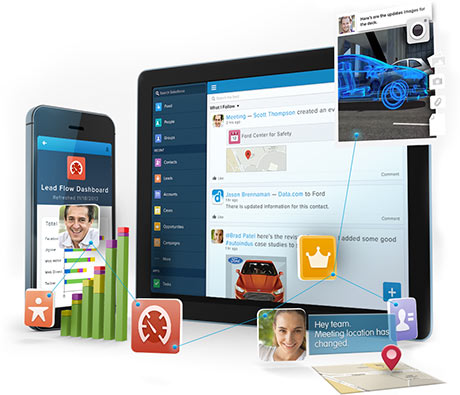
\includegraphics[width=1.00\textwidth]{ext/sf_salesCloud.jpg}
		\caption{Sales Cloud\cite{salesforce:salesCloudImg}}
		\label{fig:sf_salesCloud}
	\end{figure}

\subsubsection{Service Cloud}
Service cloud je též založen na Salesforce1 Platform. Jedná se o doručování obsahu klientům odkudkoliv a jakéhokoliv zařízení. Service Cloud je v podstatě kontejner pro rozesílání informací na sociální sítě, emailem a dalšími prostředky. Dokáže i umožnit reagovat na podněty zaslané zákazníky v jednotlivých komunikačních nástrojích.\nocite{salesforce:serviceCloud}
	\begin{figure}[htbp]
		\centering
			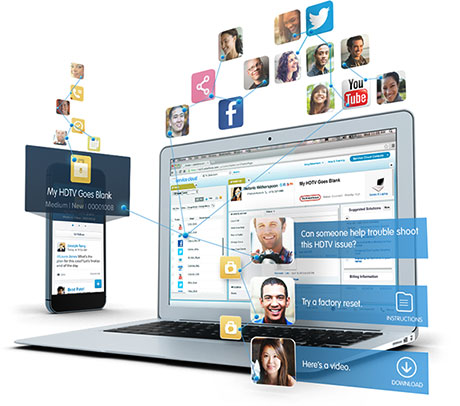
\includegraphics[width=1.00\textwidth]{ext/sf_serviceCloud.jpg}
		\caption{Service Cloud\cite{salesforce:serviceCloudImg}}
		\label{fig:sf_serviceCloud}
	\end{figure}

\subsubsection{ExactTarget Marketing Cloud}
I Marketing Cloud je založen na Salesforce1 Platform. Tato služba umožňuje obchodníkům vytvářet kampaně 1:1, tedy přímo zaměřené na každého uživatele zvlášť. Umožňuje kombinovat tradiční komunikační kanály jako email, mobilní telefon a nové sociální sítě a jakékoliv myslitelné produkty na webu.\nocite{salesforce:marketingCloud}
	\begin{figure}[htbp]
		\centering
			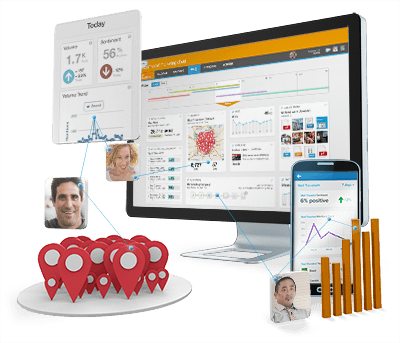
\includegraphics[width=1.00\textwidth]{ext/sf_marketingCloud.png}
		\caption{Marketing Cloud\cite{salesforce:marketingCloudImg}}
		\label{fig:sf_marketingCloud}
	\end{figure}

\subsubsection{Salesforce Platform}
Salesforce1 Platform umožňuje rychlý vývoj a nasazení aplikací. Jedná se o kompletně cloudové řešení.\nocite{salesforce:platform} Platforma umožňuje
	\begin{itemize}
		\item Vytvářet vlastní aplikace psaním kódu nebo grafickým editorem,
		\item spojení dat mezi sebou pomocí výkonného API,
		\item nasadit a zpřístupnit jakoukoliv aplikaci na Salesforce,
		\item získat a využívat předem připravené aplikace z AppExchange.
	\end{itemize}
	\begin{figure}[htbp]
		\centering
			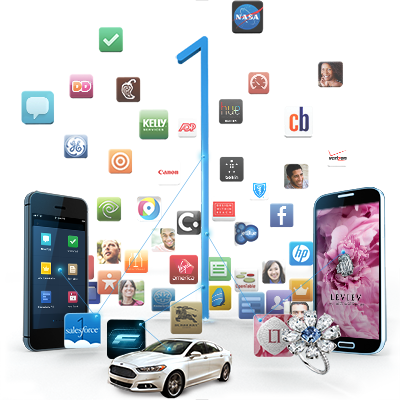
\includegraphics[width=1.00\textwidth]{ext/sf_platform.png}
		\caption{Salesforce Platform\cite{salesforce:platformImg}}
		\label{fig:sf_platform}
	\end{figure}

\subsubsection{Salesforce Chatter}
TODO
	\begin{figure}[htbp]
		\centering
			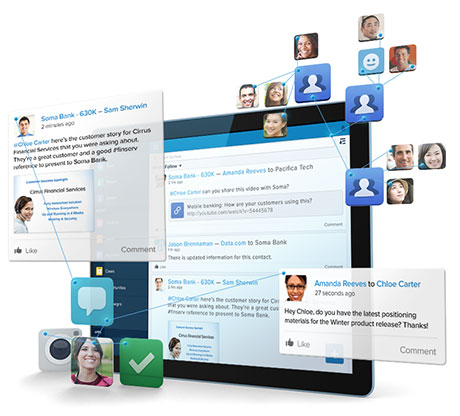
\includegraphics[width=1.00\textwidth]{ext/sf_chatter.jpg}
		\caption{Salesforce Chatter\cite{salesforce:chatterImg}}
		\label{fig:sf_chatter}
	\end{figure}

\subsubsection{Salesforce Work.com}
TODO
	\begin{figure}[htbp]
		\centering
			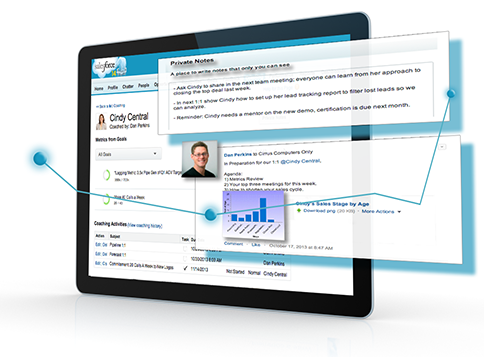
\includegraphics[width=1.00\textwidth]{ext/sf_work.png}
		\caption{Salesforce Work.com\cite{salesforce:workImg}}
		\label{fig:sf_work}
	\end{figure}

\subsection{Amazon}
Druhý zástupce cloudových služeb, patřící k těm největším dodnes. Historie služeb Amazonu sahají k téměř samotnému počátku označení cloud, do let po roce 2002. Amazon v té době spustil jejich první službu Amazon web services (AWS), což je dnes asi nejkomplexnější cloudová služba vůbec. Poskytuje nepřeberné množství služeb, od výpočetního výkonu, přes úložiště, databáze, platební systémy, přes monitorování sítě, až po "`pracovní sílu"' (inteligenci) lidí.

Pro komplexnost bych zde představil alespoň pár základních, pro tuto práci zajímavých, služeb.

\subsubsection{Elastic Compute Cloud}
EC2, jak se zkráceně označuje je pronájen výpočetního výkonu cloudu. Jedná se o pronajímané virtuální servery od čistých systémů až ke komplexním řešením s předinstalovanými aplikacemi.

\subsubsection{Simple storage service --- S3}
Nejspíše nejvyužívanější služba Amazonu. Jedná se o úložiště, tedy službu, kam můžeme nahrávat data a uskladnit je v prostoru cloudu. Jedná se o neomezené (omezením jsou finanční možnosti hostované firmy) úložiště pro libovolný obsah. Služba se dá využívat buď samostatně, jako jednoduché úložiště s poskytováním dat před HTTP, nebo jako úložiště pro ostatní služby AWS.

Další zajímavou přidanou hodnotou služby je poskytování obsahu přes distribuovanou síť BitTorrent. Pokud je tedy potřeba distribuovat obsah více příjemcům, je tato volba velice zajímavou možností. Bohužel má omezení, kdy je takto možné distribuovat soubory pouze menší 5 GB. Přesný popis je dostupný na \href{http://docs.aws.amazon.com/AmazonS3/latest/dev/S3Torrent.html}{docs.aws.amazon.com}

\subsubsection{Amazon CloudFront}
CloudFront je služba pro decentralizované distribuované dodání obsahu. Služba funguje jako CDN, kdy obsah je zrcadlen na několika serverech po celém světě a zaručuje co nejrychlejší doručení dat k uživatelům. Díky CDN se použije nejbližší geograficky, nebo nejméně vytížený server. Výhodou je i to, že je velice malá šance, že by vypadli všechny servery a obsah se tak stal úplně nedostupný, spíše naopak je zaručeno, že obsah bude velice dobře dostupný.

Jedná se tak o vyspělejší úložiště S3 se kterým tato služba spolupracuje. V S3 vyberete obsah, který se má rozdistribuovat mezi ostatní datová centra aby byl dostupnější.

\subsection{Google}
Společnost Google se zaměřuje na cloudové služby velice úzce a poskytuje široké spektrum služeb. Mezi produkty se nachází jak aplikace pro běžného uživatele až po firemní klientelu a vysoce specifické a náročné aplikace.

\subsubsection{Gmail}
Asi nejznámější cloudovou službou Google je emailová schránka. V základní verzi poskytuje 15 GB místa a přístup přes IMAP i POP3. Se schránkou automaticky uživatel získává i OpenID\footnote{OpenID je otevřený standard popisující decentralizovaný způsob autentizace uživatelů, který odstraňuje potřebu na straně provozovatele služby poskytovat a vyvíjet vlastní systémy pro autentizaci a který rovněž samotným uživatelům služby umožňuje konsolidaci jejich digitálních identit.\cite{wiki:openID}} díky kterému se může přihlašovat do dalších služeb nejen společnosti Google.
\begin{figure}[htbp]
	\centering
		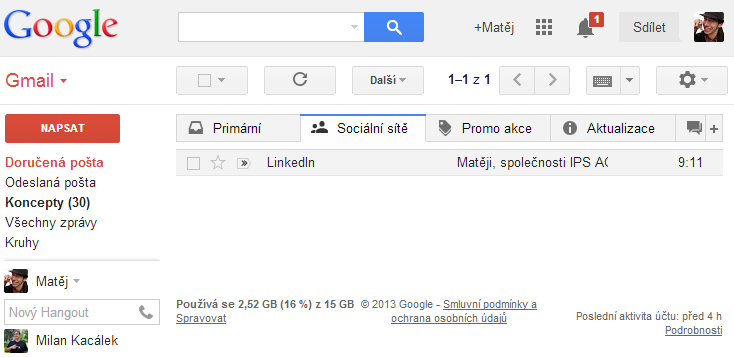
\includegraphics[width=1.00\textwidth]{ext/googleGmail.png}
	\caption{Emailová schránka Gmail}
	\label{fig:googleGmail}
\end{figure}

\subsubsection{Drive}
Aplikace Drive je cloudové úložiště pro osobní potřebu uživatele s účtem Google. V základním balíčku je diskový prostor 15 GB, který jde následně za poplatek rozšířit. Nahrané dokumenty a soubory je možné upravovat, ukládat, nebo sdílet. Je samozřejmě možné vytvářet i nové dokumenty. Dále Drive umožňuje spolupráci několika lidí na jednom dokumentu a to i zároveň.
\begin{figure}[htbp]
	\centering
		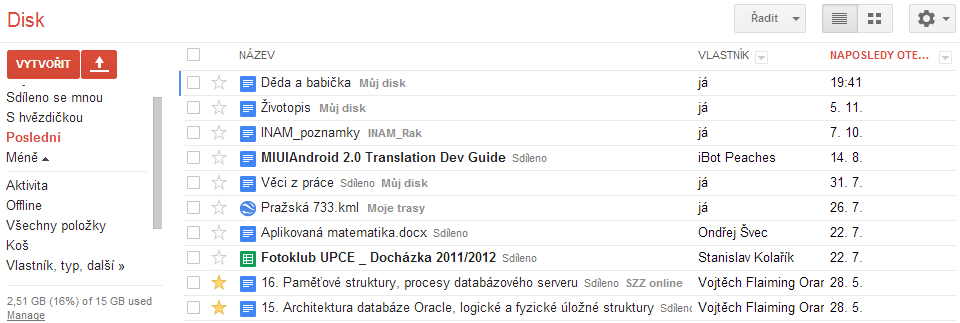
\includegraphics[width=1.00\textwidth]{ext/googleDrive.png}
	\caption{Diskové úložiště Drive}
	\label{fig:googleDrive}
\end{figure}

\subsubsection{Keep}
Aplikace Keep slouží pro uchovávání krátkých poznámek a zápisků. Služba je synchronizována mezi zařízeními K poznámkám je možné si přidat oznámení, tedy si můžete poznamenat třeba nezapomenout nakoupit pečivo a když víte, že kolem osmé budete v obchodě, aplikace na mobilním zařízení vás v tu dobu upozorní. Dále je možné vkládat k poznámkám fotky, nebo hlasový komentář.
\begin{figure}[htbp]
	\centering
		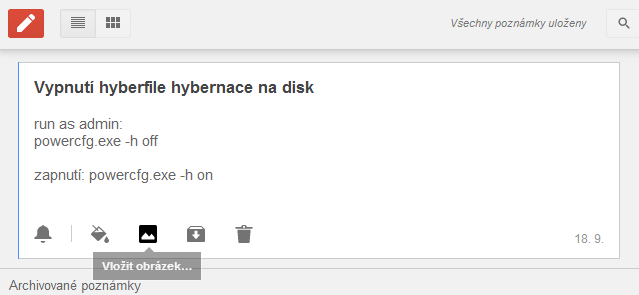
\includegraphics[width=1.00\textwidth]{ext/googleKeep.png}
	\caption{Poznámky Keep}
	\label{fig:googleKeep}
\end{figure}

\subsubsection{Enterprise}

\begin{itemize}
	\item Disk, Apps, Gmail, Hangouts
\end{itemize}
\subsubsection{Cloud Platform}
\subsubsection{Cloud Print}
\subsubsection{App Engine}
\subsubsection{Compute Engine}
\subsubsection{Cloud Storage}
\subsubsection{BigQuery}

\subsection{IBM}
\subsubsection{IBM SmartCloud Enterprise} IaaS a PaaS
\subsubsection{IBM SmartCloud Application Services}

\subsection{Microsoft}
\subsubsection{Office Web Apps}
Stejně jako jiné korporace i Microsoft má svůj vlastní kancelářský balík online. Přišel s ním sice později než konkurence, ovšem díky velice propracovanému desktopovému balíku Microsoft Office (nyní pokročilé online službě \href{https://office.microsoft.com}{Office 365}) a dlouhodobému vývoji se rozhodně \href{https://skydrive.live.com}{Office Web Apps} povedl. Webové office jsou zjednodušenou verzí plnohodnotného balíku, který je možné zakoupit.

\subsubsection{Office 365}
Office 365 je plnohodnotný cloudový kancelářský balík pro domácnosti i firmy. V tomto balíku je možné využívat všech výhod webového balíku Office Web Apps, jako sdílení dokumentů, přístup odkudkoliv, spolupráci více uživatelů a další. 

Jako nevýhodu Office 365 vidím, pokud chceme používat klasický desktopový kancelářský balík a nikoliv pouze aplikaci Office 365 ve webovém prohlížeči. V tomto případě si stále musíme zakoupit plnohodnotný kancelářský balík a do něho až následně Office 365 integrovat, což zvyšuje náklady. Otázkou však je, zda-li je klasický program stále potřeba, když je možné soubory v cloudových office editovat i bez připojení lokálně a po připojení se k Internetu soubory nahrát do úložiště.

\subsubsection{Azure}
Microsoft Azure je cloudová platforma pro vývoj vlastních aplikací. Využívá globálních datacenter společnosti Microsoft. Díky rozsáhlosti sítě a velikosti datacenter poskytuje dostatečný prostor pro škálování a možnost reagovat okamžitě na potřeby navýšení výkonu. Azure umožňuje vyvíjet webové aplikace, využívat cloudové úložiště, obří databáze v podobě Big Data. Slouží i jako platforma pro ukládání dat a přístup k datům aplikací z mobilních zařízení. Azure je možné využívat i jako distribuovanou síť pro multimediální obsah od kódování, ochranu až po streaming. \nocite{ms:azure}

\subsubsection{Intune}
Windows Intune kombinuje možnosti cloudu s on-premise infrastrukturou a nabízí řešení, které lze přizpůsobit podle vašich potřeb na správu počítačů a mobilních zařízení.\cite{ms:intune}

Jedná se tak o cloudovou službu, která umožňuje spravovat zabezpečení jednotlivých firemních zařízení a jejich přizpůsobení. Jiné zabezpečení bude kladeno na mobilní zařízení a jiná na pevné stanice v kancelářích a naprosto jiné pro samostatné firemní servery. Všechno toto nastavení lze díky Intune spravovat z jednoho místa. Služba umožňuje i snadnou distribuci aktualizací a samotného softwaru.

\subsubsection{Hyper-V}
Hyper-V je virtualizační služba, která je dostupná pro klasické počítače a nikoliv jen pro cloudové řešení. Hyper-V běží pod jedním hostitelským operačním systémem (obvykle Serverovou verzí MS Windows) a umožňuje spouštění dalších hostovaných virtuálních operačních systémů v rámci jednoho fyzického stroje.

Hyper-V je možné získat jako aplikaci instalovatelnou jako součást systému zdarma. Druhou variantou je získat Hyper-V jako samostatný celek Microsoft Hyper-V Server, který je jakožto samostatný hypervisor, bez nutnosti mít hostitelský systém, poskytován též zdarma.

\subsubsection{Dynamics CRM Online}
Jako i ostatní společnosti i Microsoft poskytuje hotové řešení pro podniky a komunikaci se zákazníky. V tomto případě se opět jedná o CRM systém s možností analyzovat trh, trendy a vývoj prodeje. Umožňuje sledovat produktivitu prodeje a díky tomu zlepšit prodej produktů.

\subsection{VMware}
\href{http://www.vmware.com/cz/products.html}{vmware produkty}
\subsubsection{vCloud Hybrid Service}
\subsubsection{vCloud}
\subsubsection{vSphere}
\subsubsection{vCenter}

\subsection{Další jiná využití cloudu}
Kromě velkých hráčů na trhu zde jsou i menší společnosti, které neposkytují komplexní služby, ale zaměřují se spíše na specifické odvětví. I mezi těmito produkty jsou ovšem velice zdařilé projekty, ač většinou k jiným účelům, než se dají použít výše zmíněné cloudové služby.

\subsubsection{Dropbox}
Dropbox je synchronizační cloudová služba a úložiště. Služba funguje na principu synchronizace všech klientských stanic a mobilních telefonů a jejich obsahu. Data jsou primárně ukládána v koncových stanicích a obsah se klonuje do úložiště dropboxu. Odtud se v případě zjištění, že na některém zařízení obsah chybí kopíruje i do něho. 

V případě mobilních zařízení se nesynchronizuje přímo, ale jako jednotlivé soubory, aby v zařízení nezabíral tolik místa a zbytečně nevytěžoval omezený a pomalý datový tarif. Služba umožňuje automaticky z mobilních zařízení synchronizovat pořízený multimediální obsah.

Další možností služby je sdílení složek mezi více uživateli služby, kdy se ostatním zobrazí obsah sdíleného adresáře se kterým následně mohou pracovat.

Služba poskytuje i přístup k historii upravených souborů -- provádí verzování známé ze systémů jako SVN nebo Git.

\begin{figure}[h]
	\centering
		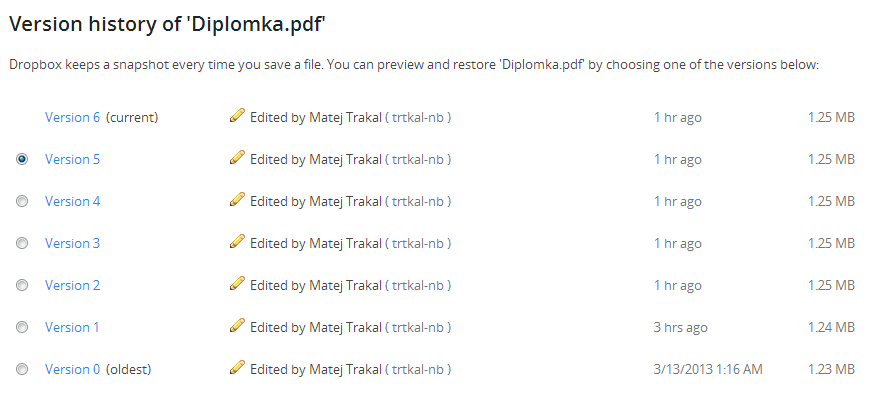
\includegraphics[width=1.00\textwidth]{ext/dropbox_versioning.png}
	\caption{Verzování ve službě dropbox}
	\label{fig:dropbox_versioning}
\end{figure}

\subsubsection{OnLive}
\label{sec:onlive}
Nabízí koncepčně naprosto jiné služby, než zde všechny zmíněné. Jedná se o službu doručování obrazu vzdáleného serveru, který funguje jako výpočetní datové centrum. V tomto centru se na farmě grafických karet a procesorů provádí vysoce náročné výpočetní operace a jejich výsledek v podobě obrazu je doručován po kvalitní datové lince k uživatelům. Služba by se dala přirovnat k funkci vzdálené plochy.

Služba aktuálně nabízí dvě varianty poskytovaného obsahu.

\paragraph{OnLive Games}
V prvním případě je doručovaný obsah zaměřen na herní průmysl, kdy se v datovém centru vypočítávají operace hry a klientovy je doručen pouze obraz v podobě snímků.
Od uživatele jde interakce na server, kde se zakomponuje pohyb jeho polohovacím zařízením do hry a obraz se změnou je opět odeslán k uživateli. V tomto případě je kladen vysoký nárok na kvalitní internetové připojení a nízkou latenci, jelikož je třeba, aby byl obraz i reakce plynulé.
\paragraph{OnLive Desktop}
Druhou variantou je služba Desktop. V tomto případě je poskytován vzdáleně operační systém společnosti Microsoft s předinstalovaným kancelářským balíkem Office. Systém běží na vysoce výkonných serverech, tedy práce s ním je plynulá a reakce okamžité. Opět zde platí podmínka na kvalitní datovou linku, ovšem již ne s tak vysokými nároky jako u výše zmiňované herní služby. Služba je zaměřena na uživatele na cestách, kdy potřebují z různých zařízení přistupovat ke svému počítači a nechtějí nebo nemohou sebou neustále brát notebook. Systém je možné spouštět i na tabletech se systémem Mac a Android.

\subsubsection{OwnCloud}
\begin{quote}ownCloud je řešení pro ukládání souborů, které můžeme nasadit ve firmě a inteligentně používat pro sdílení souborů přes internet. Nabízí ale i řadu dalších služeb (aplikací, které fungují jako zásuvné moduly), například kalendář, kontakty, úkoly a poznámky, hudební přehrávač, editor/prohlížeč obrázků, přehrávač videí, apod. K tomu se přidávají další vlastnosti jako šifrování a jednoduché verzování souborů.\cite{samuraj:ownCLoud5}
\end{quote}
TODO: přidat vlastní omáčku, spousta prostoru pro rozvedení...
\begin{figure}[htbp]
	\centering
		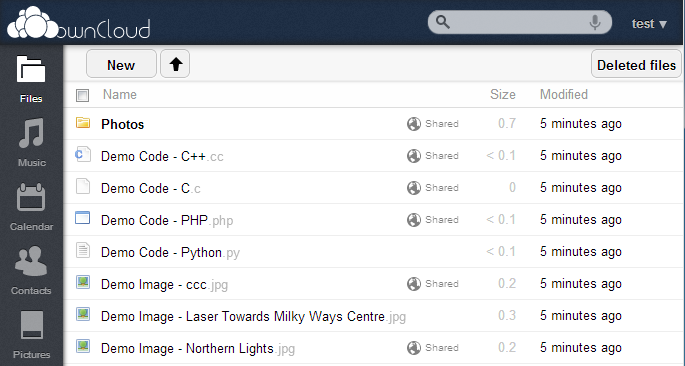
\includegraphics[width=1.00\textwidth]{ext/ownCloud.png}
	\caption{ownCloud}
	\label{fig:ownCloud}
\end{figure}

\subsubsection{Cloud9}
\href{https://github.com/ajaxorg/cloud9}{Cloud 9 IDE} je vývojové prostředí, které je poháněno javascriptovým frameworkem \href{http://nodejs.org/}{Node.js} běžícím na serveru. Jedná se tak o cloudové open source řešení vývojového prostředí. Jako základ IDE je využíváno editoru kódu \href{http://ace.c9.io/}{Ace}. Prostředí umí všechny základní věci jako zvýrazňování syntaxe, napovídání a doplňování kódu, zobrazování náhledu v případě kódu v HTML5+CSS a JavaScriptu.

Cloud9 IDE je možné využívat pro projekty na vlastním serveru, nebo využívat některého z hostingových cloudových center.

Na tomto open source IDE je založena i služba \href{https://c9.io/}{c9.io}, která kromě poskytnutí funkcí a hostování IDE umožňuje klonování projektů a spravování u nich na serveru. Možnost kompilace a deploye se spouštěním serverových částí kódu, poskytuje přístup ke konzole pomocí ssh přes webový prohlížeč (možnost používat tar, wget, git a další nástroje). Navíc služba dokáže dobře spolupracovat s verzovacími nástroji jako \href{https://github.com/}{Github}, \href{https://bitbucket.org/}{Bitbucket}, \href{http://www.windowsazure.com}{Windows Azure} a dalšími.
Dále tato služba umožňuje spolupráci více lidí nad projektem a možnost editace jednoho souboru se zvýrazněním, kde kolegové soubor právě upravují.
\begin{figure}[htbp]
	\centering
		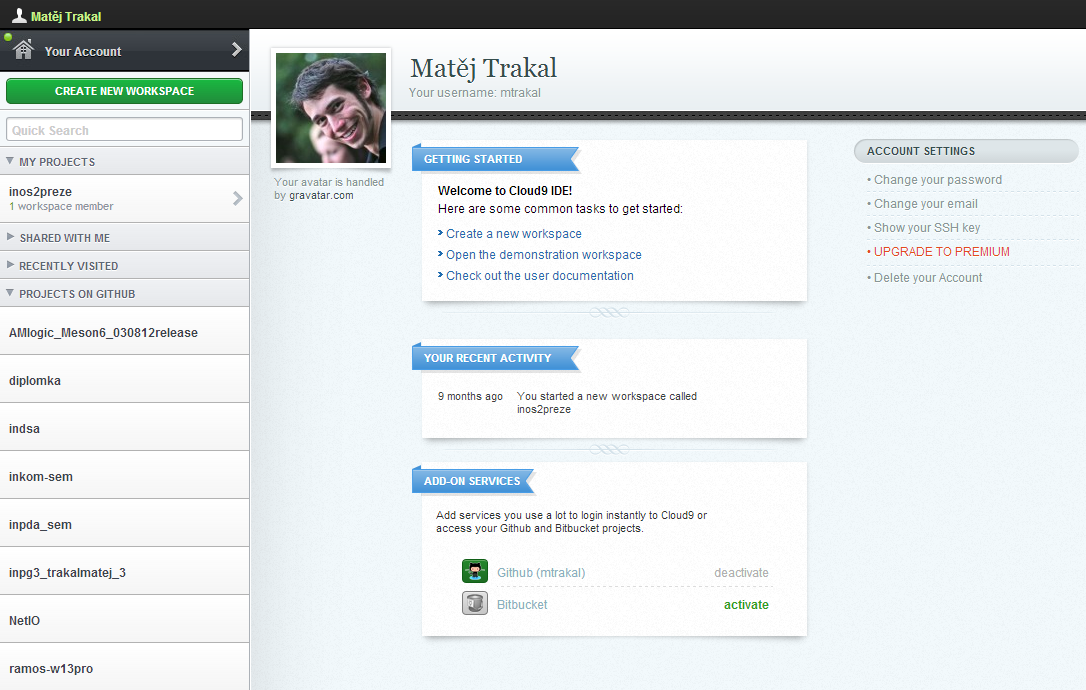
\includegraphics[width=1.00\textwidth]{ext/c9ioDashboard.png}
	\caption{c9.io dashboard}
	\label{fig:c9ioDashboard}
\end{figure}

\begin{figure}[htbp]
	\centering
		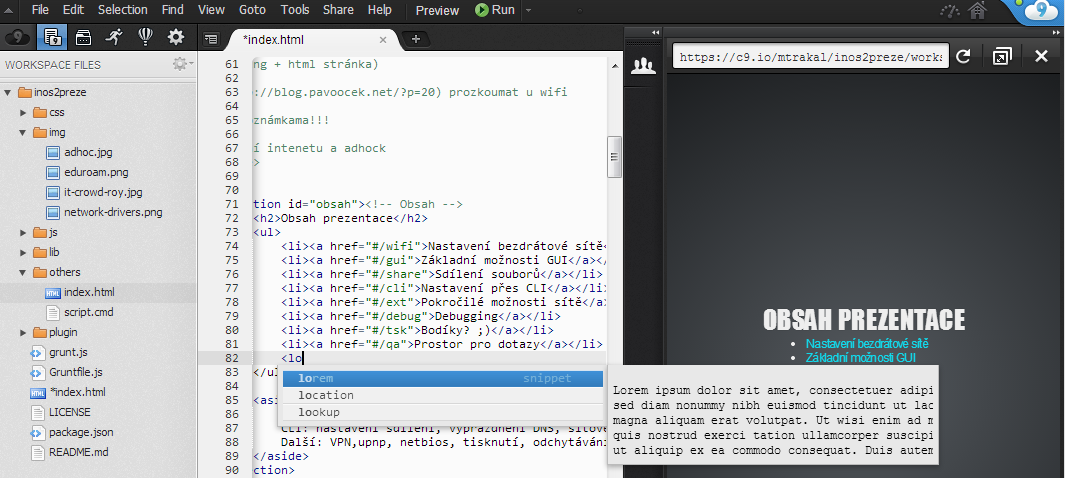
\includegraphics[width=1.00\textwidth]{ext/c9ioEditor.png}
	\caption{c9.io editor kódu s náhledem výstupu}
	\label{fig:c9ioEditor}
\end{figure}


Cloud9 využívá například i embedded zařízení \href{http://beagleboard.org/}{BeagleBoard}, ve kterém běží Linux, nebo Android OS. Díky tomuto editoru můžete programovat přímo na zařízení a okamžitě spouštět a zobrazovat výsledek. Zařízení má mnoho vstupů i výstupů a dá se na něm s přídavnými moduly sestavit v podstatě libovolná aplikace, od multimediálního centra, až po inteligentního robota na úklid domácnosti.
\begin{figure}[htbp]
	\centering
		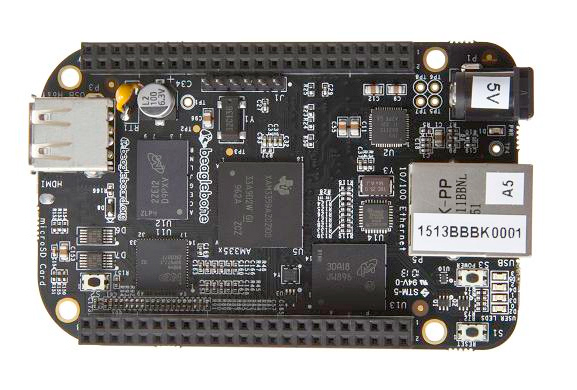
\includegraphics[width=1.00\textwidth]{ext/product_detail_black_lg_horiz.png}
	\caption{Embedded zařízení BeagleBone Black}
	\label{fig:beagleboneblack}
\end{figure}

\section{Nasazení a programování pro cloud}
TODO

\section{Popis praktické části}
TODO

\section{Závěr}

\begin{comment}
2013-01-21 http://cs.wikipedia.org/wiki/Cloud_computing
2012-12-11 http://www.lupa.cz/clanky/co-je-a-co-neni-cloud/

- historie
2013-01-29 http://technik.ihned.cz/c1-48480960-miri-pocitace-do-oblak
2013-02-20 http://www.itbiz.cz/cloud-computing-v-praxi-maly-pohled-do-historie-aneb-vse-co-jste-o-nem-chteli-vedet-ale-bali-jste-se-zeptat
2013-02-23 http://www.ddconnect.cz/brezen-2012/datova-centra.html


��tov�n� po men��ch �sec�ch ne� u hostingu, nap�. hodinov�
dynamick� zv��en� v�konu kdy� je pot�eba - virtualizace - denn� z�t�, no�n� klid, �spora financ�? Mo�n�

Cloudy:
AWS - Amazon Web Services
App Engine - Google
Azure - MS
OnLive - cloudov� vzd�len� plocha NX

http://www.zdrojak.cz/clanky/zaciname-s-node-js-na-windows-azure/
https://developers.google.com/appengine/
http://mtdiplomka.appspot.com/

2013-03-12 http://www.systemonline.cz/virtualizace/
2013-03-12 http://en.wikipedia.org/wiki/Cloud_computing_security
2013-03-12 http://www.infoworld.com/d/security-central/gartner-seven-cloud-computing-security-risks-853
2013-03-12 http://www.technologyreview.com/featuredstory/416804/security-in-the-ether/
http://www.cloud.cz/bezpenost/175-role-bezpecnosti-v-duveryhodnem-cloudu.html
http://www.itbiz.cz/cloud-computing-v-praxi-cloud-a-bezpecnost-2
2013-05-07 http://www.lupa.cz/clanky/predstaveni-cloudovych-sluzeb-amazon-web-services/
2013-05-07 http://www.zdrojak.cz/clanky/pouzivame-datove-uloziste-amazon-s3/
\end{comment}
%\section{Sezn�men� s Cloud Computingem}
%\section{Bezpe�nost a cloud}

%\section{P�vodn� vymezen� Cloud Computingu}
V p�vodn�m v�znamu slova cloud computing se uv�d�l v�znam, kter� se omezil na t�i pojmy. Jednalo se o Software, Platform a Infrastructure pod kter�ma se skr�valy pronaj�man� slu�by, kde se cena ur�ovala za v�po�tn� v�kon spot�ebovan� danou slub�nou.

Slu�bu cloud computing m��eme rozd�lit dle n�sleduj�c�ch kategori�:
\subsection{Dle podkytovan�ho obsahu}

\subsubsection{SaaS -- Software as a Service}
\subsubsection{PaaS -- Platform as a Service}
\subsubsection{IaaS -- Infrastructure as a Service}

\subsection{Dle dostupnosti slu�eb}
\subsubsection{Priv�tn�}
\subsubsection{Ve�ejn�}
\subsubsection{Hybridn�}




%!!!!!!!! ZAČÁTEK PRAKTICKÉ ČÁSTI !!!!!!!!!!
% \include{prakticka/PraktickaUvod}



% Záver
% \include{chap/Zaver}

% Seznam použité literatury (citace)
%\nocite{*} 															% vytvoří seznam literatury ze všech citací obsažených v souboru BibTeXu
%\nocite{Nobody06} 												% funguje jako \cite (přidá do soub.aux na místo, které je určeno umístěním
																					% tohoto příkazu v textu, položku), ale nevytiskne odkaz v textu
%\cite{Ceska1994} 												% vytvoří „odkaz“ do textu
%\ref{kriz} 															% křížový odkaz s odkazem na %rel
%\href{http://blog.trtkal.net}{odkaz} 		% externí odkaz
%\label{kriz} 														% popisek

%\bibliographystyle{alpha} % povolí citace pomoci BibTeXu
\DeclareUrlCommand\url{\def\UrlLeft{<}\def\UrlRight{>}\urlstyle{tt}}  %rm/sf/tt
%\renewcommand{\emph}[1]{\textsl{#1}}    	% melo by byt kurziva nebo sklonene,
%\bibliographystyle{bib/csplainnat/csplainnat}
\bibliographystyle{bib/czechiso/czechiso} 		% zapne podporu pro citace pomocí normy ČSN ISO 690 a ČSN ISO 690-2
\def\refname{Použitá literatura}
\bibliography{bib/Citace} 								% odkaz na soubor s citacema (*.bib)

% Přílohy
%\include{chap/Prilohy}


% KONEC DOKUMENTU
\end{document}

% vyplnění řádku / zarovnání více textů na řádek
% První \hfill druhý \\První \hrulefill druhý \\Třetí \dotfill a \dotfill čtvrtý

\begin{comment}
	Příkaz Anglická verze Česká verze  
	\abstractname  Abstract  Abstrakt  
	\alsoseename  see also  viz také  
	\appendixname  Appendix  Příloha  
	\bibname  Bibliography  Literatura  
	\ccname  cc  Na vědomí  (u~dopisů) 
	\chaptername  Chapter  Kapitola  
	\contentsname  Contents  Obsah  
	\enclname  encl  Příloha  (u~dopisů) 
	\figurename  Figure  Obrázek  
	\headtoname  To  Komu  (u~dopisů) 
	\indexname  Index  Rejstřík  
	\listfigurename  List of Figures  Seznam obrázků  
	\listtablename  List of Tables  Seznam tabulek  
	\partname  Part  Část  
	\prefacename  Preface  Předmluva  
	\refname  References  Reference  
	\seename  see  viz  
	\tablename  Table  Tabulka 
\end{comment}